% Options for packages loaded elsewhere
\PassOptionsToPackage{unicode}{hyperref}
\PassOptionsToPackage{hyphens}{url}
%
\documentclass[
]{article}
\usepackage{lmodern}
\usepackage{amssymb,amsmath}
\usepackage{ifxetex,ifluatex}
\ifnum 0\ifxetex 1\fi\ifluatex 1\fi=0 % if pdftex
  \usepackage[T1]{fontenc}
  \usepackage[utf8]{inputenc}
  \usepackage{textcomp} % provide euro and other symbols
\else % if luatex or xetex
  \usepackage{unicode-math}
  \defaultfontfeatures{Scale=MatchLowercase}
  \defaultfontfeatures[\rmfamily]{Ligatures=TeX,Scale=1}
\fi
% Use upquote if available, for straight quotes in verbatim environments
\IfFileExists{upquote.sty}{\usepackage{upquote}}{}
\IfFileExists{microtype.sty}{% use microtype if available
  \usepackage[]{microtype}
  \UseMicrotypeSet[protrusion]{basicmath} % disable protrusion for tt fonts
}{}
\makeatletter
\@ifundefined{KOMAClassName}{% if non-KOMA class
  \IfFileExists{parskip.sty}{%
    \usepackage{parskip}
  }{% else
    \setlength{\parindent}{0pt}
    \setlength{\parskip}{6pt plus 2pt minus 1pt}}
}{% if KOMA class
  \KOMAoptions{parskip=half}}
\makeatother
\usepackage{xcolor}
\IfFileExists{xurl.sty}{\usepackage{xurl}}{} % add URL line breaks if available
\IfFileExists{bookmark.sty}{\usepackage{bookmark}}{\usepackage{hyperref}}
\hypersetup{
  pdftitle={Report 1},
  pdfauthor={Klaudia Balcer},
  hidelinks,
  pdfcreator={LaTeX via pandoc}}
\urlstyle{same} % disable monospaced font for URLs
\usepackage[margin=1in]{geometry}
\usepackage{color}
\usepackage{fancyvrb}
\newcommand{\VerbBar}{|}
\newcommand{\VERB}{\Verb[commandchars=\\\{\}]}
\DefineVerbatimEnvironment{Highlighting}{Verbatim}{commandchars=\\\{\}}
% Add ',fontsize=\small' for more characters per line
\usepackage{framed}
\definecolor{shadecolor}{RGB}{248,248,248}
\newenvironment{Shaded}{\begin{snugshade}}{\end{snugshade}}
\newcommand{\AlertTok}[1]{\textcolor[rgb]{0.94,0.16,0.16}{#1}}
\newcommand{\AnnotationTok}[1]{\textcolor[rgb]{0.56,0.35,0.01}{\textbf{\textit{#1}}}}
\newcommand{\AttributeTok}[1]{\textcolor[rgb]{0.77,0.63,0.00}{#1}}
\newcommand{\BaseNTok}[1]{\textcolor[rgb]{0.00,0.00,0.81}{#1}}
\newcommand{\BuiltInTok}[1]{#1}
\newcommand{\CharTok}[1]{\textcolor[rgb]{0.31,0.60,0.02}{#1}}
\newcommand{\CommentTok}[1]{\textcolor[rgb]{0.56,0.35,0.01}{\textit{#1}}}
\newcommand{\CommentVarTok}[1]{\textcolor[rgb]{0.56,0.35,0.01}{\textbf{\textit{#1}}}}
\newcommand{\ConstantTok}[1]{\textcolor[rgb]{0.00,0.00,0.00}{#1}}
\newcommand{\ControlFlowTok}[1]{\textcolor[rgb]{0.13,0.29,0.53}{\textbf{#1}}}
\newcommand{\DataTypeTok}[1]{\textcolor[rgb]{0.13,0.29,0.53}{#1}}
\newcommand{\DecValTok}[1]{\textcolor[rgb]{0.00,0.00,0.81}{#1}}
\newcommand{\DocumentationTok}[1]{\textcolor[rgb]{0.56,0.35,0.01}{\textbf{\textit{#1}}}}
\newcommand{\ErrorTok}[1]{\textcolor[rgb]{0.64,0.00,0.00}{\textbf{#1}}}
\newcommand{\ExtensionTok}[1]{#1}
\newcommand{\FloatTok}[1]{\textcolor[rgb]{0.00,0.00,0.81}{#1}}
\newcommand{\FunctionTok}[1]{\textcolor[rgb]{0.00,0.00,0.00}{#1}}
\newcommand{\ImportTok}[1]{#1}
\newcommand{\InformationTok}[1]{\textcolor[rgb]{0.56,0.35,0.01}{\textbf{\textit{#1}}}}
\newcommand{\KeywordTok}[1]{\textcolor[rgb]{0.13,0.29,0.53}{\textbf{#1}}}
\newcommand{\NormalTok}[1]{#1}
\newcommand{\OperatorTok}[1]{\textcolor[rgb]{0.81,0.36,0.00}{\textbf{#1}}}
\newcommand{\OtherTok}[1]{\textcolor[rgb]{0.56,0.35,0.01}{#1}}
\newcommand{\PreprocessorTok}[1]{\textcolor[rgb]{0.56,0.35,0.01}{\textit{#1}}}
\newcommand{\RegionMarkerTok}[1]{#1}
\newcommand{\SpecialCharTok}[1]{\textcolor[rgb]{0.00,0.00,0.00}{#1}}
\newcommand{\SpecialStringTok}[1]{\textcolor[rgb]{0.31,0.60,0.02}{#1}}
\newcommand{\StringTok}[1]{\textcolor[rgb]{0.31,0.60,0.02}{#1}}
\newcommand{\VariableTok}[1]{\textcolor[rgb]{0.00,0.00,0.00}{#1}}
\newcommand{\VerbatimStringTok}[1]{\textcolor[rgb]{0.31,0.60,0.02}{#1}}
\newcommand{\WarningTok}[1]{\textcolor[rgb]{0.56,0.35,0.01}{\textbf{\textit{#1}}}}
\usepackage{longtable,booktabs}
% Correct order of tables after \paragraph or \subparagraph
\usepackage{etoolbox}
\makeatletter
\patchcmd\longtable{\par}{\if@noskipsec\mbox{}\fi\par}{}{}
\makeatother
% Allow footnotes in longtable head/foot
\IfFileExists{footnotehyper.sty}{\usepackage{footnotehyper}}{\usepackage{footnote}}
\makesavenoteenv{longtable}
\usepackage{graphicx,grffile}
\makeatletter
\def\maxwidth{\ifdim\Gin@nat@width>\linewidth\linewidth\else\Gin@nat@width\fi}
\def\maxheight{\ifdim\Gin@nat@height>\textheight\textheight\else\Gin@nat@height\fi}
\makeatother
% Scale images if necessary, so that they will not overflow the page
% margins by default, and it is still possible to overwrite the defaults
% using explicit options in \includegraphics[width, height, ...]{}
\setkeys{Gin}{width=\maxwidth,height=\maxheight,keepaspectratio}
% Set default figure placement to htbp
\makeatletter
\def\fps@figure{htbp}
\makeatother
\setlength{\emergencystretch}{3em} % prevent overfull lines
\providecommand{\tightlist}{%
  \setlength{\itemsep}{0pt}\setlength{\parskip}{0pt}}
\setcounter{secnumdepth}{-\maxdimen} % remove section numbering
\usepackage{bbm}
\usepackage{caption}
\usepackage{tabularx}
\usepackage{booktabs}
\usepackage{graphicx}
\usepackage{amsmath}

\title{Report 1}
\usepackage{etoolbox}
\makeatletter
\providecommand{\subtitle}[1]{% add subtitle to \maketitle
  \apptocmd{\@title}{\par {\large #1 \par}}{}{}
}
\makeatother
\subtitle{Multiple Regression and Multiple Testing}
\author{Klaudia Balcer}
\date{12/17/2021}

\begin{document}
\maketitle

{
\setcounter{tocdepth}{3}
\tableofcontents
}
\pagebreak

\hypertarget{introduction}{%
\section{Introduction}\label{introduction}}

Linear regression is a basic statistical method. It can model linear
dependencies well. However, it is also prone to noise. Including to many
variables in the model may cause a bad reality mapping. A simple way to
select variables which should be included in the model is multiple
testing. In this report we will show a simulation study on the
efficiency of this approach. The structure of the document is as
folllows. In the first section we will introduce the subject of multiple
regression. After that we will focus on multiple testing in the second
section. The third sections contains the theoretical calculations and
results obtained from the simulation study.

\hypertarget{multiple-regression}{%
\section{Multiple Regression}\label{multiple-regression}}

Multiple Linear Regression is a statistical approach for modeling a
linear relationship between a scalar response variable and many
explanatory variables. Let's consider \(n\) observations (values of
response variable and vectors of explanatory variables). The number of
explanatory variables is denoted by \(p-1\). The model is of the form:

\[Y_i = \beta_0 + X_i\beta_{[1, \ldots,p-1]} + \epsilon_i\] or
equivalently the model in a matrix form:

\[Y = X\beta + \epsilon\] where:

\begin{itemize}
\item
  \(Y_i\) is the value of the response variable for \(i\)th observation,
  \(Y\) is the (horizontal) vector of response variable
  (\(n \times 1\));
\item
  \(X_i\) is the (vertical) vector of explanatory variables for \(i\)th
  observation, \(X\) is a design matrix (first column filled with ones,
  \(X_{i, j+1}\) is the value of the \(j\)th explanatory variable in the
  \(i\)th observation (\(n \times p\));
\item
  \(\beta_0\) is the intercept,
\item
  \(\beta\) is the (horizontal) vector of coefficients (\(n \times 1\)),
\item
  \(\epsilon_i\) is the error for \(i\)th observation, let's consider
  normally distributed errors:
  \(\epsilon_i \sim \mathcal N (0, \sigma^2)\), \(\epsilon\) is the
  vector of errors (\(n \times 1\)),
\item
  \(i\) is the index of the observation.
\end{itemize}

There are two standard formulas for estimating \(\beta\): least squares
and maximum likelihood. When the error is normally distributed (as we
have previously assumed) those method are equivalent.

The estimator of \(\beta\) is denoted by \(b\), the estimator of
\(\sigma\) (standard deviation of the errors) will be denoted as \(s\).

The fitted values of the response variables will be denoted as
\(\hat{Y}\). We can calculate it by replacing \(\beta\) with its
estimator and \(\epsilon\) by its mean value (\(b\) and \(0\)).

\[\hat Y = Xb\] The difference between real and fitted (predicted)
values of the response variable is called residual and it is marked with
\(e\):

\[e = Y - \hat Y\] Let's get into more details.

\hypertarget{estimating-regression-coefficients}{%
\subsection{Estimating Regression
Coefficients}\label{estimating-regression-coefficients}}

We will show the least squares estimation of \(\beta\). The method is
based on minimalizing the values of the error \(\epsilon\).

\[b = arg\min_{b \in \mathbb R ^n}  \quad (Y - Xb)^T(Y - Xb)\]

Let's expand the minimised formula:

\[(Y - Xb)^T(Y - Xb) = Y^TY - b^TX^TY - Y^TXb + b^TX^TXb\]

Let's derive by \(b\):

\[-X^TY - Y^TX + 2X^TXb = 0\]

\[X^TXb = X^TY\] The sationar point:

\[b = (X^TX)^{-1}X^TY\] The second derivative is \(2X^TX\). Let's have
\(v \in \mathbb R ^p\).

\[v^T X^TXv = (Xv)^TXv = Xv \circ Xv = \Vert Xv \Vert^2 \geq 0\]

Thus, \(X^TX\) is a positive-definite matrix, so we have found the local
minimum.

Let take a look on the distribution of the estimator:

\[b \sim \mathcal N\big(\beta, \sigma^2(X^TX)^{-1}\big)\]

\hypertarget{fitted-values}{%
\subsection{Fitted Values}\label{fitted-values}}

After providing the formula for \(b\) we are able to derive the formula
for \(\hat Y\) in terms of \(X\) and \(Y\):

\[\hat Y = Xb = X(X^TX)^{-1}X^TY\]

As we can see in the above equation, there is a linear dependence
between \(Y\) and \(\hat Y\). The matrix transforming \(Y\) into
\(\hat Y\) is called hat matrix and it is denoted by \(H\):

\[\hat Y = H Y\] The formual for the hat matrix is:

\[H = X(X^TX)^{-1}X^T\]

THe matrix \(H\) \emph{projects} \(Y\) into \(\hat Y\).

\hypertarget{estimator-of-sigma}{%
\subsection{\texorpdfstring{Estimator of
\(\sigma\)}{Estimator of \textbackslash sigma}}\label{estimator-of-sigma}}

The estimator of \(\sigma^2\) uses the values of the residuals has the
form:

\[s^2 = \frac {e^Te} {n-p} = \frac {(Y - Xb)^T(Y - Xb)} {n-p}\]

\hypertarget{wishart-and-inverse-wishart-distribution}{%
\subsection{Wishart and Inverse-Wishart
Distribution}\label{wishart-and-inverse-wishart-distribution}}

In the upcoming simulations, we will consider the design matrix of
i.i.d. normally distributed random variables. X is a \(n \times p\)
matrix, each row is independently drawn from p-variate normal
distribution with mean zero and covariance matrix
\(\Sigma = \frac 1 {1000}I\). Thus, \(X^TX\) (\(p \times p\) random
matrix) has the Wishart probability distribution with parameters
\(\Sigma\) and \(n\):

\[X^TX \sim W_p(\Sigma, n)\]

Thus, the inverse of \(X^TX\) comes from the Inverse-Wishart
distribution:

\[(X^TX)^{-1} \sim W_p^{-1} (\Sigma^{-1}, n)\]

The mean value of a random variable from Inverse-Wishart distribution
has the mean:

\[\mathbb E \big[(X^TX)^{-1} \big] = \frac {\Sigma^{-1}} {n - p - 1}\]

\hypertarget{multiple-testing}{%
\section{Multiple Testing}\label{multiple-testing}}

Let's consider p testing problems:

\[H_{0, i}: \mu_i = 0 \quad vs \quad H_{1, i}: \mu_i \neq 0\]

Multiple testing means testing many individual hypotheses (\(H_{0, i}\)
vs.~\(H_{1, i}\)) at the same time. To simply statistically test each
hypothesis separately doesn't lead to satisfying results. We use
\textbf{multiple comparison procedures} (MCPs) instead. MCPs are used to
improve the quality of the tests.

The outcome of an MCP can be presented in the following form:

\begin{longtable}[]{@{}llll@{}}
\toprule
& accepted & rejected & total\tabularnewline
\midrule
\endhead
true & TN (U) & FP (S) & \(p_0\)\tabularnewline
false & FN (V) & TP (T) & \(p - p_0\)\tabularnewline
total & p - R & R & p\tabularnewline
\bottomrule
\end{longtable}

The symbols used:

\begin{itemize}
\item
  TN - True Negatives - the null hypothesis is true, and it was accepted
  (U in \emph{Candes}),
\item
  FP - False Positives - the null hypothesis is true, but it was
  rejected (V in \emph{Candes}),
\item
  FN - False Negatives - the null hypothesis is false, and it was
  accepted (T in \emph{Candes}),
\item
  TP - True Positives - the null hypothesis is false, and it was
  rejected (S in \emph{Candes}),
\item
  \(p_0\) - the number of true null hypotheses,
\item
  R - the number of rejected hypotheses,
\item
  \(p\) - the number of hypotheses.
\end{itemize}

\hypertarget{test-quality-measures}{%
\subsection{Test Quality Measures}\label{test-quality-measures}}

The definition of the Type I Error does not simply propagate to multiple
testing problem. On the one hand, allowing a single false discovery with
the probability \(\alpha\) is a very strict condition. On the other
hand, allowing the probability of false discovery in each test to be
\(\alpha\), leads to many false discoveries. Hence we need to introduce
new quality measures: FWER and FDR.

\hypertarget{fwer}{%
\subsubsection{FWER}\label{fwer}}

FWER stands for \textbf{F}amili\textbf{w}ise \textbf{E}rror
\textbf{R}ate.

In \textbf{strong} sense: it is the probability of making any false
discoveries:

\[FWER = \mathbb{P}(V \geq 1)\]

In \textbf{weak} sense: it is the probability of making any false
discoveries if all the global null hypothesis is true:

\[FWER = \mathbb{P}(V \geq 1 |  \forall_i H_{0, i})\]

\hypertarget{fdr}{%
\subsubsection{FDR}\label{fdr}}

FDR stands for \textbf{F}alse \textbf{D}iscovery \textbf{R}ate id the
expected value of FDP (\textbf{F}alse \textbf{D}iscovery
\textbf{P}roportion) - the ratio between the numbers of false
discoveries and all rejections:

\[FDR = \mathbb{E}\Bigg[ \frac{FP}{ max(R, 1)}\Bigg]\] Under the global
null hypothesis, FDR and FWEAR are equivalent.

\hypertarget{mfdr}{%
\subsubsection{mFDR}\label{mfdr}}

\[mFDR = \frac {\mathbb E V } {\mathbb E R} = \frac {\mathbb E V} {\mathbb E [V + T]} \]

\hypertarget{power}{%
\subsubsection{Power}\label{power}}

Power is the probability of rejecting the null hypothesis when it is
false. In the above terms, we can express it as the expected value of
the ratio of TP and the number of false hypotheses:

\[power = \mathbb{E}\Bigg[ \frac{TP}{p - p_0} \Bigg]\]

\hypertarget{multiple-testing-procedures}{%
\subsection{Multiple Testing
Procedures}\label{multiple-testing-procedures}}

For all below procedures, first we calculate the p-values of single
tests:

\begin{itemize}
\item
  p-values: \(p_1, p_2, \ldots, p_p\),
\item
  ordered p-values: \(p_{(1)}, p_{(2)}, \ldots, p_{(p)}\).
\end{itemize}

\hypertarget{bonferronis-procedure}{%
\subsubsection{Bonferroni's procedure}\label{bonferronis-procedure}}

Reject \(H_{0, i}\) if: \[p_i <  \frac \alpha n\]

This method is very conservative. We know from the lecture that
Bonferroni's method controls FWER in a strong sense. In fact,

\[FWER = \mathbb{P}(FP \geq 1) \leq \sum_{i=1}^{p_0}\mathbb P(FP = i) = \sum_{i=1}^{n_0} {{p_0}\choose{i}} \alpha^i(1 - \alpha)^{p_0 - i}\]

\[FWER \leq \frac{p_0}{p} \alpha\]

\hypertarget{benjamini-hochbergs-procedure}{%
\subsubsection{Benjamini-Hochberg's
procedure}\label{benjamini-hochbergs-procedure}}

Reject \(H_{0, (i)}\) if:

\[\exists _{(j \geq i)}  \quad p_{(j)} <  \frac {j} {n} \alpha\]
Benjamini-Hochberg's method is a step-down procedure. This procedure
controls FDR under independence. Thus, it controls FWER weakly. It does
not control FWER in a strong sense. It is much more liberal than
Hochberg's procedure (more powerful and leads to more false
discoveries).

\hypertarget{simualtions}{%
\section{Simualtions}\label{simualtions}}

\hypertarget{theoretical-calculations}{%
\subsection{Theoretical calculations}\label{theoretical-calculations}}

\hypertarget{variance-of-the-estimators-of-individual-regression-coefficients}{%
\subsubsection{Variance of the Estimators of Individual Regression
Coefficients}\label{variance-of-the-estimators-of-individual-regression-coefficients}}

For a fixed matrix of observation \(X\), the variance of the estimators
of individual regression coefficients is given by the formula:

\[\sigma_{\beta_i}^2 = \sigma^2(X^TX)^{-1}_{[i, i]}\]

When resampling the matrix of observations \(X\), we replace
\((X^TX)^{-1}_{[i, i]}\) by its expectation:

\[\mathbb E_X \sigma_{\beta_i}^2 = \sigma^2\mathbb E \Big[(X^TX)^{-1}_{[i, i]}\Big]\]
We know that \((X^TX)^{-1}\) has the inverse-Wishart distribution. Its
expected value is given by the formula:

\[\mathbb E \big[ (X^TX)^{-1} \big]= \frac {n \mathbb I_{n \times n}}{n - p - 1}\]

Thus:

\[\mathbb E_X \sigma_{\beta_i}^2 = \sigma^2\mathbb E \Big[(X^TX)^{-1}_{[i, i]}\Big] = \sigma^2 \frac {n}{n-p-1}\]
\textbf{1. n = 10}

\[\mathbb E_X \sigma_{\beta_i}^2 = \sigma^2 \frac {n}{n-p-1} = 1 \cdot \frac {1000} {1000 - 9} = \frac {1000}{991} \approx 1.01\]

\textbf{2. n = 100}

\[\mathbb E_X \sigma_{\beta_i}^2 = \sigma^2 \frac {n}{n-p-1} = 1 \cdot \frac {1000} {1000 - 99} = \frac{1000}{901} \approx 1.11\]

\textbf{3. n = 500}

\[\mathbb E_X \sigma_{\beta_i}^2 = \sigma^2 \frac {n}{n-p-1} = 1 \cdot \frac {1000} {1000 - 499} = \frac {1000} {501} \approx 2.00\]

\textbf{4. n = 950}

\[\mathbb E_X \sigma_{\beta_i}^2 = \sigma^2 \frac {n}{n-p-1} = 1 \cdot \frac {1000} {1000 - 949} = \frac {1000}{51} \approx 19.61\]

We expect the variance of the estimators to be very large for p close to
n.~Thus, the results of the experiment are expected to be not satisfying
for p close to n.

\hypertarget{fwer-1}{%
\subsubsection{FWER}\label{fwer-1}}

\[FWER = \mathbb P (V > 0) = \mathbb P (FP > 0) = \mathbb P \Big(\bigcup_{i \in \mathcal H_0} V_i \Big)\]

When having fixed observation matrix \(X\) it is hard to provide the
exact formula for FWER. However, we can easily derive an upper bound:

\[FWER = \mathbb P \Big(\bigcup_{i \in \mathcal H_0} V_i \Big) \leq \sum_{i \in \mathcal H_0} \mathbb P(V_i) = p_0 \cdot \alpha\]

When resampling the observations matrix, the individuial regression
coeficients become independent:

\[\mathbb E_X \hat \beta \sim \mathcal N \big(\beta, \sigma^2 \mathbb E (X^TX^{-1})\big) = \mathcal N \big(\beta, \sigma^2 \frac {n\mathbb I}{n - p  - 1}\big) \]

Whis leads us to a formuka for FWER:

\[\mathbb E_X FWER = \mathbb P \Big(\bigcup_{i \in \mathcal H_0} \mathbb E _XV_i \Big) = 1 - \mathbb P \Big(\bigcap_{i \in \mathcal H_0} \mathbb E _XV_i \Big) = 1 - (1 - \alpha)^{p_0}\]

\textbf{n = 10}

\begin{displaymath} 
 \mathbb E_X FWER = 1 - (1 - \alpha)^{p_0} = 1 - (1 - \alpha)^{p_0} \approx 0.41
\end{displaymath}

\textbf{n = 100}

\begin{displaymath} 
 \mathbb E_X FWER = 1 - (1 - \alpha)^{p_0} = 1 - (1 - \alpha)^{p_0} \approx 0.41
\end{displaymath}

\textbf{n = 500}

\begin{displaymath} 
 \mathbb E_X FWER = 1 - (1 - \alpha)^{p_0} = 1 - (1 - \alpha)^{p_0} \approx 0.41
\end{displaymath}

\textbf{n = 950}

\begin{displaymath} 
 \mathbb E_X FWER = 1 - (1 - \alpha)^{p_0} = 1 - (1 - \alpha)^{p_0} \approx 0.41
\end{displaymath}

The construction of Bonferroni's procedure changes the rejection
threshold. Whus, we can derive the formula for FWER in a similar way:

\[FWER = \mathbb P \Big(\bigcup_{i \in \mathcal H_0} V_i \Big) \leq \sum_{i \in \mathcal H_0} \mathbb P(V_i) = p_0 \cdot \frac \alpha n\]

\[\mathbb E_X FWER = \mathbb P \Big(\bigcup_{i \in \mathcal H_0} \mathbb E _XV_i \Big) = 1 - \mathbb P \Big(\bigcap_{i \in \mathcal H_0} \mathbb E _XV_i \Big) = 1 - \prod_{i \in \mathcal H_0}\mathbb  P \big(\mathbb E_X V_i\big) = 1 - \Big(1 - \frac \alpha n\Big)^{p_0}\]

\textbf{n = 10}

\begin{displaymath} 
 \mathbb E_X FWER = 1 - \Big(1 - \frac \alpha n\Big)^{p_0} = 1 - \Big(1 - \frac {0.1} {10} \Big)^{5} = 1 - 0.99^5 \approx 0.05
\end{displaymath}

\textbf{n = 100}

\begin{displaymath} 
 \mathbb E_X FWER = 1 - \Big(1 - \frac \alpha n\Big)^{p_0} = 1 - \Big(1 - \frac {0.1} {100} \Big)^{5} = 1 - 0.999^5 \approx 0
\end{displaymath}

\textbf{n = 500}

\begin{displaymath} 
 \mathbb E_X FWER = 1 - \Big(1 - \frac \alpha n\Big)^{p_0} = 1 - \Big(1 - \frac {0.1} {500} \Big)^{5} = 1 - 0.9998^5 \approx 0
\end{displaymath}

\textbf{n = 950}

\begin{displaymath} 
 \mathbb E_X FWER = 1 - \Big(1 - \frac \alpha n\Big)^{p_0} = 1 - \Big(1 - \frac {0.1} {950} \Big)^{5} = 1 - 0.9998947^5 \approx 0
\end{displaymath}

For Benjamini-Hochberg:

\[FWER = \mathbb P \Big(\bigcup_{i \in \mathcal H_0} V_i \Big) \leq \sum_{i \in \mathcal H_0} \mathbb P(V_i) = \sum_{i = 6}^{p} \mathbb P(V_i)\]

\[\mathbb E_X FWER = \mathbb P \Big(\bigcup_{i \in \mathcal H_0} \mathbb E _XV_i \Big) = 1 - \mathbb P \Big(\bigcap_{i \in \mathcal H_0} \mathbb E _XV_i \Big) = 1 - \prod_{i \in \mathcal H_0}\mathbb  P \big(\mathbb E_X V_i\big)  = 1 - \prod_{i = 6}^p\mathbb  P \big(\mathbb E_X V_i\big)\]

The exact value of \(\mathbb P(V_i)\) and \(\mathbb P(\mathbb E_X V_i)\)
depends on the order of p values.

\hypertarget{power-1}{%
\subsubsection{Power}\label{power-1}}

Test statistics: \(Z = \frac {\hat \beta} {\sigma_{\beta_i}}\). We
reject the null hypothesis when \(|Z| > \Phi^{-1}(1 - \frac \alpha 2)\).

\[power = \mathbb P(V_i | H_{0,  1}^c) = \mathbb P \Big(|Z| > \Phi^{-1}(1  - \frac \alpha 2)\Big) = \mathbb P \Big(Z > \Phi^{-1}(1  - \frac \alpha 2)\Big) + \mathbb P \Big(Z < - \Phi^{-1}(1  - \frac \alpha 2)\Big)\]

Let's standarize the \(Z\) statistics:

\[power = \mathbb P \Big(\frac{Z - 3}{\sigma_{\beta_i}} > \frac{\Phi^{-1}(1  - \frac \alpha 2)\sigma_{\beta_i} - 3}{\sigma_{\beta_i}}\Big) + \mathbb P \Big(\frac{Z - 3}{\sigma_{\beta_i}} < \frac{-\Phi^{-1}(1  - \frac \alpha 2)\sigma_{\beta_i} - 3}{\sigma_{\beta_i}}\Big)\]
\[power = 1 - \Phi\Big(\frac{\Phi^{-1}(1  - \frac \alpha 2)\sigma_{\beta_i} - 3}{\sigma_{\beta_i}}  \Big) + \Phi\Big(\frac{-\Phi^{-1}(1  - \frac \alpha 2)\sigma_{\beta_i} - 3}{\sigma_{\beta_i}} \Big)\]
\textbf{n = 10}

\begin{displaymath} power = 1 - \Phi\Big(\frac{\Phi^{-1}(1  - \frac \alpha 2) - 3}{\sigma_{\beta_i}}  \Big) + \Phi\Big( \frac{-\Phi^{-1}(1  - \frac \alpha 2) - 3} {\sigma_{\beta_i}} \Big) = 
  \end{displaymath}
\begin{displaymath}1 - \Phi\Big(\frac{\Phi^{-1}(1  - \frac \alpha 2) - 3}{ \frac {1000}{\sqrt{989}} }  \Big) + \Phi\Big( \frac{-\Phi^{-1}(1  - \frac \alpha 2) - 3} {\frac {1000}{\sqrt{989}}} \Big) \approx 0.84
\end{displaymath}

\textbf{n = 100}

\begin{displaymath} power = 1 - \Phi\Big(\frac{\Phi^{-1}(1  - \frac \alpha 2) - 3}{\sigma_{\beta_i}}  \Big) + \Phi\Big( \frac{-\Phi^{-1}(1  - \frac \alpha 2) - 3} {\sigma_{\beta_i}} \Big) = 
  \end{displaymath}
\begin{displaymath}1 - \Phi\Big(\frac{\Phi^{-1}(1  - \frac \alpha 2) - 3}{ \frac {1000}{\sqrt{899}} }  \Big) + \Phi\Big( \frac{-\Phi^{-1}(1  - \frac \alpha 2) - 3} {\frac {1000}{\sqrt{899}}} \Big) \approx 0.81
\end{displaymath}

\textbf{n = 500}

\begin{displaymath} power = 1 - \Phi\Big(\frac{\Phi^{-1}(1  - \frac \alpha 2) - 3}{\sigma_{\beta_i}}  \Big) + \Phi\Big( \frac{-\Phi^{-1}(1  - \frac \alpha 2) - 3} {\sigma_{\beta_i}} \Big) = 
  \end{displaymath}
\begin{displaymath}1 - \Phi\Big(\frac{\Phi^{-1}(1  - \frac \alpha 2) - 3}{ \frac {1000}{\sqrt{499}} }  \Big) + \Phi\Big( \frac{-\Phi^{-1}(1  - \frac \alpha 2) - 3} {\frac {1000}{\sqrt{499}}} \Big) \approx 0.64
\end{displaymath}

\textbf{n = 950}

\begin{displaymath} power = 1 - \Phi\Big(\frac{\Phi^{-1}(1  - \frac \alpha 2) - 3}{\sigma_{\beta_i}}  \Big) + \Phi\Big( \frac{-\Phi^{-1}(1  - \frac \alpha 2) - 3} {\sigma_{\beta_i}} \Big) = 
  \end{displaymath}
\begin{displaymath}1 - \Phi\Big(\frac{\Phi^{-1}(1  - \frac \alpha 2) - 3}{ \frac {1000}{\sqrt{49}} }  \Big) + \Phi\Big( \frac{-\Phi^{-1}(1  - \frac \alpha 2) - 3} {\frac {1000}{\sqrt{49}}} \Big) \approx 0.78
\end{displaymath}

\hypertarget{mfdr-1}{%
\subsubsection{mFDR}\label{mfdr-1}}

\[FDR = \mathbb E \frac  {V}{max(R,  1)}\]

\[mFDR = \frac  { \mathbb E V}{max( \mathbb E R,  1)} = \frac  { \mathbb E \Big[ \sum_{i \in \mathcal H_0} V_i \Big]}{max\Big( \mathbb E \big[ \sum_{i = 1}^p R \big],  1\Big)} = \frac  {\sum_{i \in \mathcal H_0} \mathbb E \Big[  V_i \Big]}{max\Big(  \sum_{i \in \mathcal H_0}\mathbb E  R + \sum_{i \in \mathcal H_0^c} \mathbb E R ,  1\Big)}  = \frac{p_0 \cdot \alpha}{max\big(p_0 \cdot \alpha + (p - p_0) \cdot power, 1 \big)}\]

\hypertarget{single-simualtion}{%
\subsection{Single simualtion}\label{single-simualtion}}

In this report we will consider data from the model:

\[Y = X\beta + \epsilon\]

where \(\beta_1 = \ldots = \beta_5 = 3\),
\(\beta_6 = \ldots=\beta_{950} = 0\),
\(X_{i, j} \sim \mathcal{N}(0, \frac 1 {1000})\) and
\(\epsilon \sim \mathcal N (0, I)\).

We will estimate the coefficients using 1000 observations.

\begin{Shaded}
\begin{Highlighting}[]
\NormalTok{alpha <-}\StringTok{ }\FloatTok{0.1}
\NormalTok{beta_vec <-}\StringTok{ }\KeywordTok{c}\NormalTok{(}\KeywordTok{rep}\NormalTok{(}\DecValTok{3}\NormalTok{, }\DecValTok{5}\NormalTok{), }\KeywordTok{rep}\NormalTok{(}\DecValTok{0}\NormalTok{, }\DecValTok{945}\NormalTok{))}
\NormalTok{X <-}\StringTok{ }\KeywordTok{matrix}\NormalTok{(}\KeywordTok{rnorm}\NormalTok{(}\DecValTok{1000} \OperatorTok{*}\StringTok{ }\DecValTok{950}\NormalTok{, }\DecValTok{0}\NormalTok{, }\KeywordTok{sqrt}\NormalTok{(}\DecValTok{1}\OperatorTok{/}\DecValTok{1000}\NormalTok{)), }\DataTypeTok{nrow=}\DecValTok{1000}\NormalTok{)}
\NormalTok{Y <-}\StringTok{ }\NormalTok{X }\OperatorTok\StringTok{ }\NormalTok{beta_vec }\OperatorTok{+}\StringTok{ }\KeywordTok{rnorm}\NormalTok{(}\DecValTok{1000}\NormalTok{, }\DecValTok{0}\NormalTok{, }\DecValTok{1}\NormalTok{)}

\NormalTok{bonferroni <-}\StringTok{ }\ControlFlowTok{function}\NormalTok{(pvals, }\DataTypeTok{alpha=}\FloatTok{0.05}\NormalTok{) \{}
\NormalTok{  n <-}\StringTok{ }\KeywordTok{length}\NormalTok{(pvals)}
\NormalTok{  pvals }\OperatorTok{<}\StringTok{ }\NormalTok{(alpha }\OperatorTok{/}\StringTok{ }\NormalTok{n)}
\NormalTok{\}}

\NormalTok{benjamini_hochberg <-}\StringTok{ }\ControlFlowTok{function}\NormalTok{(pvals, }\DataTypeTok{alpha=}\FloatTok{0.05}\NormalTok{) \{}
\NormalTok{  n <-}\StringTok{ }\KeywordTok{length}\NormalTok{(pvals)}
\NormalTok{  ord <-}\StringTok{ }\KeywordTok{order}\NormalTok{(pvals)}
\NormalTok{  ord2 <-}\StringTok{ }\KeywordTok{order}\NormalTok{(ord)}
\NormalTok{  res <-( pvals[ord] }\OperatorTok{<}\StringTok{ }\NormalTok{((alpha }\OperatorTok{*}\StringTok{ }\KeywordTok{seq}\NormalTok{(n) }\OperatorTok{/}\StringTok{ }\NormalTok{n)))}
  \KeywordTok{sapply}\NormalTok{(}\DecValTok{1}\OperatorTok{:}\NormalTok{n, }\ControlFlowTok{function}\NormalTok{(i) }\KeywordTok{any}\NormalTok{(res[i}\OperatorTok{:}\NormalTok{n]))[ord2]}
\NormalTok{\}}

\NormalTok{results <-}\StringTok{ }\KeywordTok{data.frame}\NormalTok{()}

\ControlFlowTok{for}\NormalTok{ (i }\ControlFlowTok{in} \KeywordTok{c}\NormalTok{(}\DecValTok{10}\NormalTok{, }\DecValTok{100}\NormalTok{, }\DecValTok{500}\NormalTok{, }\DecValTok{950}\NormalTok{)) \{}
\NormalTok{  model <-}\StringTok{ }\KeywordTok{lm}\NormalTok{(Y}\OperatorTok{~}\NormalTok{X[, }\DecValTok{1}\OperatorTok{:}\NormalTok{i] }\OperatorTok{-}\StringTok{ }\DecValTok{1}\NormalTok{)}
\NormalTok{  msum <-}\StringTok{ }\KeywordTok{summary}\NormalTok{(model)}
\NormalTok{  pvals <-}\StringTok{ }\NormalTok{msum}\OperatorTok{$}\NormalTok{coefficients[, }\DecValTok{4}\NormalTok{]}
  
  \CommentTok{# a)}
\NormalTok{  significance <-}\StringTok{ }\NormalTok{pvals }\OperatorTok{<}\StringTok{ }\NormalTok{alpha}
  
  \CommentTok{# b)}
  \CommentTok{# }\AlertTok{TODO}\CommentTok{: z definicji}
\NormalTok{  sd_val <-}\StringTok{ }\KeywordTok{mean}\NormalTok{(msum}\OperatorTok{$}\NormalTok{coefficients[, }\DecValTok{2}\NormalTok{])  }
\NormalTok{  CI_len <-}\StringTok{ }\KeywordTok{mean}\NormalTok{(}\KeywordTok{abs}\NormalTok{(}\KeywordTok{confint}\NormalTok{(model, }\DataTypeTok{level=}\FloatTok{0.9}\NormalTok{)[, }\DecValTok{1}\NormalTok{] }\OperatorTok{-}\StringTok{ }\KeywordTok{confint}\NormalTok{(model, }\DataTypeTok{level=}\FloatTok{0.9}\NormalTok{)[, }\DecValTok{2}\NormalTok{]))}
  
  \CommentTok{# c)}
\NormalTok{  res_i <-}\StringTok{ }\NormalTok{pvals }\OperatorTok{<=}\StringTok{ }\NormalTok{alpha}
\NormalTok{  i_TP <-}\StringTok{ }\KeywordTok{sum}\NormalTok{(res_i[}\DecValTok{1}\OperatorTok{:}\NormalTok{i] }\OperatorTok{&}\StringTok{ }\NormalTok{(beta_vec[}\DecValTok{1}\OperatorTok{:}\NormalTok{i] }\OperatorTok{>}\StringTok{ }\DecValTok{0}\NormalTok{))}
\NormalTok{  i_FP <-}\StringTok{ }\KeywordTok{sum}\NormalTok{(res_i[}\DecValTok{1}\OperatorTok{:}\NormalTok{i] }\OperatorTok{&}\StringTok{ }\NormalTok{(beta_vec[}\DecValTok{1}\OperatorTok{:}\NormalTok{i] }\OperatorTok{==}\StringTok{ }\DecValTok{0}\NormalTok{))}
  
\NormalTok{  res_ii <-}\StringTok{ }\KeywordTok{bonferroni}\NormalTok{(pvals, alpha)}
\NormalTok{  ii_TP <-}\StringTok{ }\KeywordTok{sum}\NormalTok{(res_ii[}\DecValTok{1}\OperatorTok{:}\NormalTok{i] }\OperatorTok{&}\StringTok{ }\NormalTok{(beta_vec[}\DecValTok{1}\OperatorTok{:}\NormalTok{i] }\OperatorTok{>}\StringTok{ }\DecValTok{0}\NormalTok{))}
\NormalTok{  ii_FP <-}\StringTok{ }\KeywordTok{sum}\NormalTok{(res_ii[}\DecValTok{1}\OperatorTok{:}\NormalTok{i] }\OperatorTok{&}\StringTok{ }\NormalTok{(beta_vec[}\DecValTok{1}\OperatorTok{:}\NormalTok{i] }\OperatorTok{==}\StringTok{ }\DecValTok{0}\NormalTok{))}
  
\NormalTok{  res_iii <-}\StringTok{ }\KeywordTok{benjamini_hochberg}\NormalTok{(pvals, alpha)}
\NormalTok{  iii_TP <-}\StringTok{ }\KeywordTok{sum}\NormalTok{(res_iii[}\DecValTok{1}\OperatorTok{:}\NormalTok{i] }\OperatorTok{&}\StringTok{ }\NormalTok{(beta_vec[}\DecValTok{1}\OperatorTok{:}\NormalTok{i] }\OperatorTok{>}\StringTok{ }\DecValTok{0}\NormalTok{))}
\NormalTok{  iii_FP <-}\StringTok{ }\KeywordTok{sum}\NormalTok{(res_iii[}\DecValTok{1}\OperatorTok{:}\NormalTok{i] }\OperatorTok{&}\StringTok{ }\NormalTok{(beta_vec[}\DecValTok{1}\OperatorTok{:}\NormalTok{i] }\OperatorTok{==}\StringTok{ }\DecValTok{0}\NormalTok{))}
  
\NormalTok{  results <-}\StringTok{ }\KeywordTok{rbind}\NormalTok{(results, }\KeywordTok{c}\NormalTok{(sd_val, CI_len, i_TP, i_FP, ii_TP, ii_FP, iii_TP, iii_FP))}
\NormalTok{\}}
\KeywordTok{colnames}\NormalTok{(results) <-}\StringTok{  }\KeywordTok{c}\NormalTok{(}\StringTok{"sd"}\NormalTok{, }\StringTok{"CI len"}\NormalTok{, }\StringTok{"TP"}\NormalTok{, }\StringTok{"FP"}\NormalTok{, }\StringTok{"Bonf TP"}\NormalTok{, }\StringTok{"Bonf FP"}\NormalTok{, }\StringTok{"BH TP"}\NormalTok{, }\StringTok{"BH FP"}\NormalTok{)}
\KeywordTok{rownames}\NormalTok{(results) <-}\StringTok{ }\KeywordTok{c}\NormalTok{(}\DecValTok{10}\NormalTok{, }\DecValTok{100}\NormalTok{, }\DecValTok{500}\NormalTok{, }\DecValTok{950}\NormalTok{)}
\KeywordTok{kable}\NormalTok{(results, }\DataTypeTok{digits =} \DecValTok{3}\NormalTok{)}
\end{Highlighting}
\end{Shaded}

\begin{longtable}[]{@{}lrrrrrrrr@{}}
\toprule
& sd & CI len & TP & FP & Bonf TP & Bonf FP & BH TP & BH
FP\tabularnewline
\midrule
\endhead
10 & 0.996 & 3.280 & 4 & 0 & 2 & 0 & 3 & 0\tabularnewline
100 & 1.048 & 3.452 & 5 & 6 & 1 & 0 & 1 & 0\tabularnewline
500 & 1.398 & 4.608 & 2 & 47 & 0 & 0 & 0 & 0\tabularnewline
950 & 4.391 & 14.717 & 1 & 105 & 0 & 0 & 0 & 0\tabularnewline
\bottomrule
\end{longtable}

\hypertarget{estimation}{%
\subsection{Estimation}\label{estimation}}

We will run 500 simulations.

\begin{Shaded}
\begin{Highlighting}[]
\NormalTok{FWER <-}\StringTok{ }\ControlFlowTok{function}\NormalTok{(true_values, test_results) \{ }
  \CommentTok{# T - reject H0, F - accept H0}
  \KeywordTok{as.integer}\NormalTok{(}\KeywordTok{any}\NormalTok{(test_results[}\KeywordTok{which}\NormalTok{(}\OperatorTok{!}\NormalTok{true_values)]))}
\NormalTok{\}}

\NormalTok{FDR <-}\StringTok{ }\ControlFlowTok{function}\NormalTok{(true_values, test_results) \{}
  \KeywordTok{sum}\NormalTok{(test_results[}\KeywordTok{which}\NormalTok{(}\OperatorTok{!}\NormalTok{true_values)]) }\OperatorTok{/}\StringTok{ }\KeywordTok{max}\NormalTok{(}\KeywordTok{sum}\NormalTok{(test_results), }\DecValTok{1}\NormalTok{)}
\NormalTok{\}}

\NormalTok{power <-}\StringTok{ }\ControlFlowTok{function}\NormalTok{(true_values, test_results) \{}
  \KeywordTok{mean}\NormalTok{(test_results[}\KeywordTok{which}\NormalTok{(true_values)])}
\NormalTok{\}}

\NormalTok{sim_step <-}\StringTok{ }\ControlFlowTok{function}\NormalTok{(i, X, Y) \{}
\NormalTok{  model <-}\StringTok{ }\KeywordTok{lm}\NormalTok{(Y}\OperatorTok{~}\NormalTok{X[, }\DecValTok{1}\OperatorTok{:}\NormalTok{i] }\OperatorTok{-}\StringTok{ }\DecValTok{1}\NormalTok{)}
\NormalTok{  msum <-}\StringTok{ }\KeywordTok{summary}\NormalTok{(model)}
  \CommentTok{# a}
\NormalTok{  sd_val <-}\StringTok{ }\NormalTok{msum}\OperatorTok{$}\NormalTok{coefficients[, }\DecValTok{2}\NormalTok{]}
  \CommentTok{# separatly}
  \CommentTok{# b}
\NormalTok{  CI_len <-}\StringTok{ }\KeywordTok{abs}\NormalTok{(}\KeywordTok{confint}\NormalTok{(model, }\DataTypeTok{level=}\FloatTok{0.9}\NormalTok{)[, }\DecValTok{1}\NormalTok{] }\OperatorTok{-}\StringTok{ }\KeywordTok{confint}\NormalTok{(model, }\DataTypeTok{level=}\FloatTok{0.9}\NormalTok{)[, }\DecValTok{2}\NormalTok{])}
  \CommentTok{# c}
\NormalTok{  pvals <-}\StringTok{ }\NormalTok{msum}\OperatorTok{$}\NormalTok{coefficients[, }\DecValTok{4}\NormalTok{]}
\NormalTok{  res_i <-}\StringTok{ }\NormalTok{pvals }\OperatorTok{<=}\StringTok{ }\NormalTok{alpha}
\NormalTok{  res_ii <-}\StringTok{ }\KeywordTok{bonferroni}\NormalTok{(pvals, alpha)}
\NormalTok{  res_iii <-}\StringTok{ }\KeywordTok{benjamini_hochberg}\NormalTok{(pvals, alpha)}
\NormalTok{  true_vals <-}\StringTok{ }\NormalTok{beta_vec[}\DecValTok{1}\OperatorTok{:}\NormalTok{i] }\OperatorTok{>}\StringTok{ }\DecValTok{0}
  
\NormalTok{  FWER_i <-}\StringTok{ }\KeywordTok{FWER}\NormalTok{(true_vals, res_i)}
\NormalTok{  FDR_i <-}\StringTok{ }\KeywordTok{FDR}\NormalTok{(true_vals, res_i)}
\NormalTok{  power_i <-}\StringTok{ }\KeywordTok{power}\NormalTok{(true_vals, res_i)}
  
\NormalTok{  FWER_ii <-}\StringTok{ }\KeywordTok{FWER}\NormalTok{(true_vals, res_ii)}
\NormalTok{  FDR_ii <-}\StringTok{ }\KeywordTok{FDR}\NormalTok{(true_vals, res_ii)}
\NormalTok{  power_ii <-}\StringTok{ }\KeywordTok{power}\NormalTok{(true_vals, res_ii)}
  
\NormalTok{  FWER_iii <-}\StringTok{ }\KeywordTok{FWER}\NormalTok{(true_vals, res_iii)}
\NormalTok{  FDR_iii <-}\StringTok{ }\KeywordTok{FDR}\NormalTok{(true_vals, res_iii)}
\NormalTok{  power_iii <-}\StringTok{ }\KeywordTok{power}\NormalTok{(true_vals, res_iii)}
  
  \KeywordTok{return}\NormalTok{(}\KeywordTok{list}\NormalTok{(}\DataTypeTok{sd =}\NormalTok{ sd_val, }\DataTypeTok{CI =}\NormalTok{ CI_len, }
              \DataTypeTok{FWER_st =}\NormalTok{ FWER_i, }\DataTypeTok{FDR_st =}\NormalTok{ FDR_i, }\DataTypeTok{power_st =}\NormalTok{ power_i,}
              \DataTypeTok{FWER_bonf =}\NormalTok{ FWER_ii, }\DataTypeTok{FDR_bonf =}\NormalTok{ FDR_ii, }\DataTypeTok{power_bonf =}\NormalTok{ power_ii,}
              \DataTypeTok{FWER_bh =}\NormalTok{ FWER_iii, }\DataTypeTok{FDR_bh =}\NormalTok{ FDR_iii, }\DataTypeTok{power_bh =}\NormalTok{ power_iii))}
\NormalTok{\}}

\NormalTok{i_vec <-}\StringTok{ }\KeywordTok{c}\NormalTok{(}\DecValTok{10}\NormalTok{, }\DecValTok{100}\NormalTok{, }\DecValTok{500}\NormalTok{, }\DecValTok{950}\NormalTok{)}

\NormalTok{simulation <-}\StringTok{ }\ControlFlowTok{function}\NormalTok{() \{}
\NormalTok{  X <-}\StringTok{ }\KeywordTok{matrix}\NormalTok{(}\KeywordTok{rnorm}\NormalTok{(}\DecValTok{1000} \OperatorTok{*}\StringTok{ }\DecValTok{950}\NormalTok{, }\DecValTok{0}\NormalTok{, }\KeywordTok{sqrt}\NormalTok{(}\DecValTok{1}\OperatorTok{/}\DecValTok{1000}\NormalTok{)), }\DataTypeTok{nrow=}\DecValTok{1000}\NormalTok{)}
\NormalTok{  Y <-}\StringTok{ }\NormalTok{X }\OperatorTok\StringTok{ }\NormalTok{beta_vec }\OperatorTok{+}\StringTok{ }\KeywordTok{rnorm}\NormalTok{(}\DecValTok{1000}\NormalTok{, }\DecValTok{0}\NormalTok{, }\DecValTok{1}\NormalTok{)}
  \KeywordTok{sapply}\NormalTok{(i_vec, }\ControlFlowTok{function}\NormalTok{(i) }\KeywordTok{sim_step}\NormalTok{(i, X, Y))}
\NormalTok{\}}

\NormalTok{results <-}\StringTok{ }\KeywordTok{replicate}\NormalTok{(}\DecValTok{500}\NormalTok{, }\KeywordTok{simulation}\NormalTok{())}

\NormalTok{tab <-}\StringTok{ }\KeywordTok{data.frame}\NormalTok{()}

\ControlFlowTok{for}\NormalTok{ (i }\ControlFlowTok{in} \DecValTok{1}\OperatorTok{:}\KeywordTok{length}\NormalTok{(i_vec)) \{}
\NormalTok{  sd_means <-}\StringTok{ }\KeywordTok{rowMeans}\NormalTok{(}\KeywordTok{simplify2array}\NormalTok{(results[}\DecValTok{1}\NormalTok{, i, ]))}
  
  \KeywordTok{print}\NormalTok{(}\KeywordTok{ggplot}\NormalTok{() }\OperatorTok{+}\StringTok{ }
\StringTok{    }\KeywordTok{geom_histogram}\NormalTok{(}\KeywordTok{aes}\NormalTok{(}\DataTypeTok{x=}\NormalTok{sd_means)) }\OperatorTok{+}\StringTok{ }
\StringTok{      }\KeywordTok{ggtitle}\NormalTok{(}\KeywordTok{str_c}\NormalTok{(}\StringTok{"Standard Deviation Histogram for i = "}\NormalTok{,}
                    \KeywordTok{as.character}\NormalTok{(i_vec[i]))))}
    
\NormalTok{  CI_means <-}\StringTok{ }\KeywordTok{rowMeans}\NormalTok{(}\KeywordTok{simplify2array}\NormalTok{(results[}\DecValTok{2}\NormalTok{, i, ]))}
  
  \KeywordTok{print}\NormalTok{(}\KeywordTok{ggplot}\NormalTok{() }\OperatorTok{+}
\StringTok{    }\KeywordTok{geom_histogram}\NormalTok{(}\KeywordTok{aes}\NormalTok{(}\DataTypeTok{x=}\NormalTok{CI_means)) }\OperatorTok{+}
\StringTok{      }\KeywordTok{ggtitle}\NormalTok{(}\KeywordTok{str_c}\NormalTok{(}\StringTok{"Confidence Interval Length Histogram for i = "}\NormalTok{,  }
                    \KeywordTok{as.character}\NormalTok{(i_vec[i])))) }
  
\NormalTok{  FWERv <-}\StringTok{ }\KeywordTok{mean}\NormalTok{(}\KeywordTok{simplify2array}\NormalTok{(results[}\DecValTok{3}\NormalTok{,  i, ]))}
\NormalTok{  FDRv <-}\StringTok{ }\KeywordTok{mean}\NormalTok{(}\KeywordTok{simplify2array}\NormalTok{(results[}\DecValTok{4}\NormalTok{,  i, ]))}
\NormalTok{  powerv <-}\StringTok{ }\KeywordTok{mean}\NormalTok{(}\KeywordTok{simplify2array}\NormalTok{(results[}\DecValTok{5}\NormalTok{,  i, ]))}
\NormalTok{  FWERb <-}\StringTok{ }\KeywordTok{mean}\NormalTok{(}\KeywordTok{simplify2array}\NormalTok{(results[}\DecValTok{6}\NormalTok{,  i, ]))}
\NormalTok{  FDRb <-}\StringTok{ }\KeywordTok{mean}\NormalTok{(}\KeywordTok{simplify2array}\NormalTok{(results[}\DecValTok{7}\NormalTok{,  i, ]))}
\NormalTok{  powerb <-}\StringTok{ }\KeywordTok{mean}\NormalTok{(}\KeywordTok{simplify2array}\NormalTok{(results[}\DecValTok{8}\NormalTok{,  i, ]))}
\NormalTok{  FWERbh <-}\StringTok{ }\KeywordTok{mean}\NormalTok{(}\KeywordTok{simplify2array}\NormalTok{(results[}\DecValTok{9}\NormalTok{,  i, ]))}
\NormalTok{  FDRbh <-}\StringTok{ }\KeywordTok{mean}\NormalTok{(}\KeywordTok{simplify2array}\NormalTok{(results[}\DecValTok{10}\NormalTok{,  i, ]))}
\NormalTok{  powerbh <-}\StringTok{ }\KeywordTok{mean}\NormalTok{(}\KeywordTok{simplify2array}\NormalTok{(results[}\DecValTok{11}\NormalTok{,  i, ]))}
  
\NormalTok{  tab <-}\StringTok{ }\KeywordTok{rbind}\NormalTok{(tab, }\KeywordTok{c}\NormalTok{(i_vec[i], }\KeywordTok{mean}\NormalTok{(sd_means), }\KeywordTok{mean}\NormalTok{(CI_means), FWERv, FDRv, powerv,}
\NormalTok{                      FWERb, FDRb, powerb,  FWERbh, FDRbh, powerbh))}
  
\NormalTok{\}}
\end{Highlighting}
\end{Shaded}

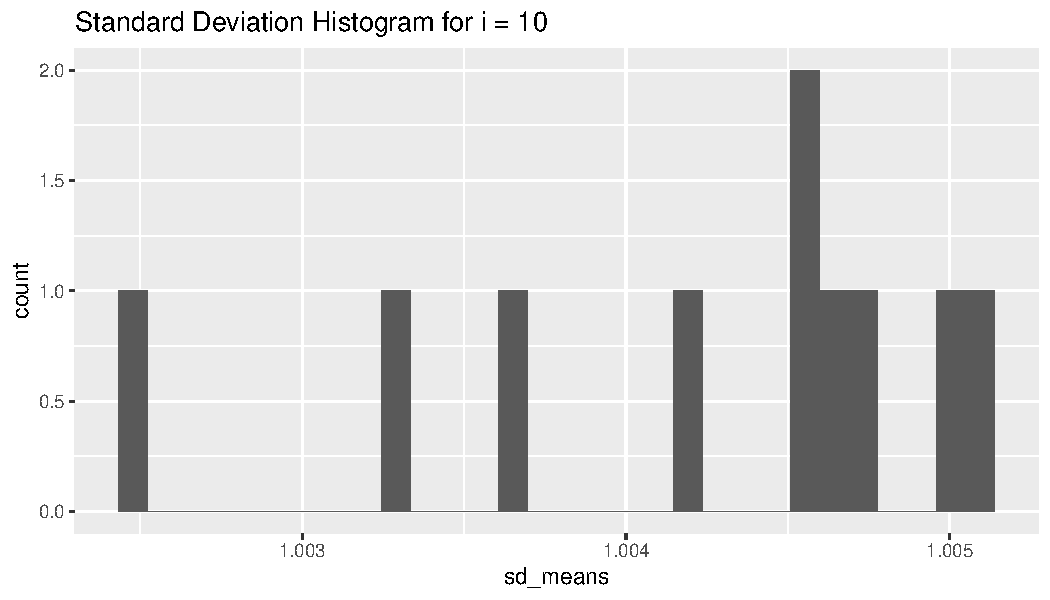
\includegraphics{report_files/figure-latex/task_2-1.pdf}
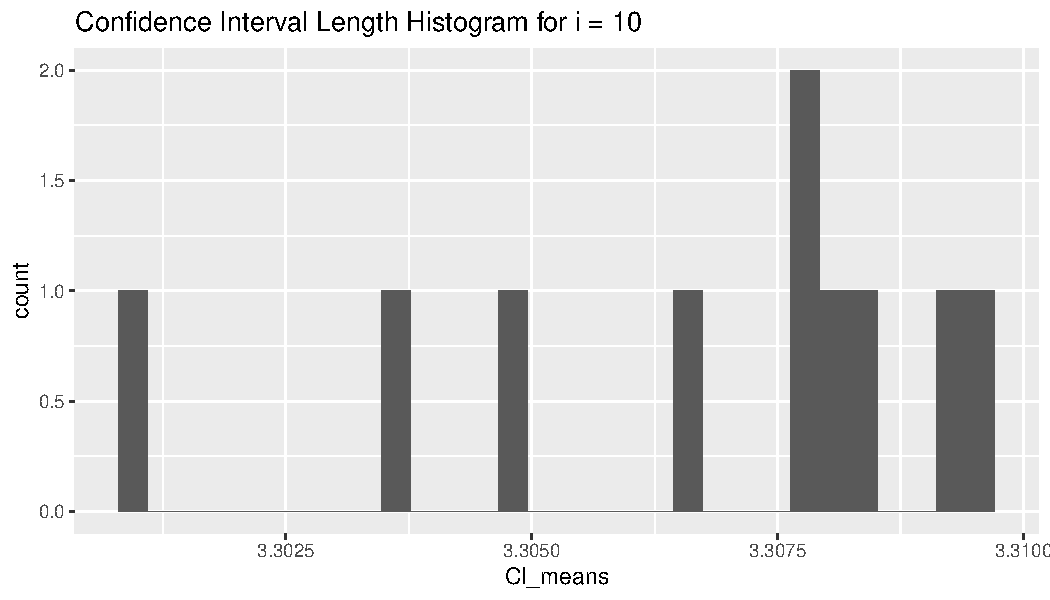
\includegraphics{report_files/figure-latex/task_2-2.pdf}
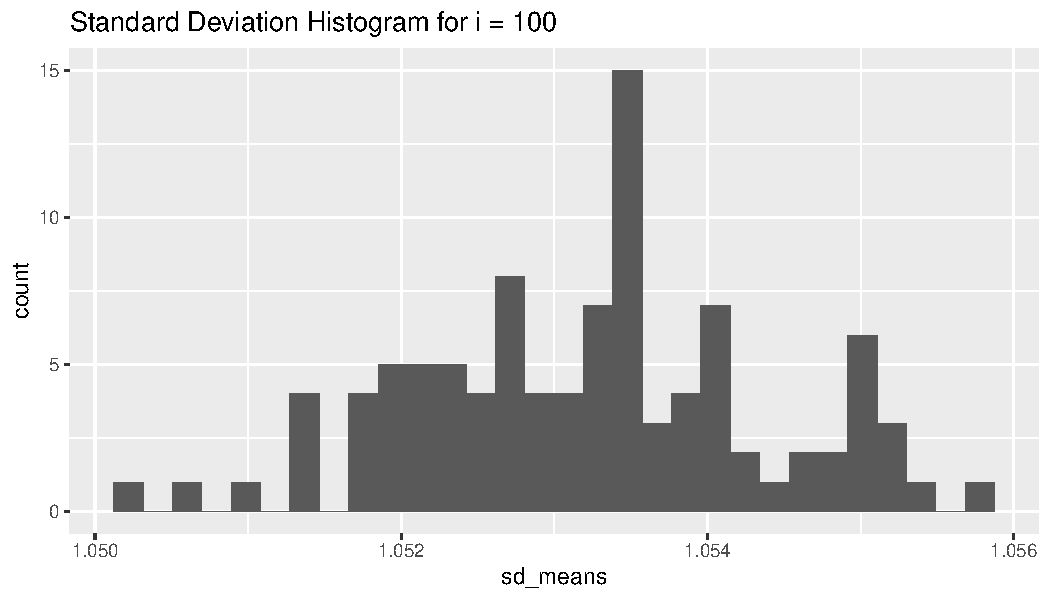
\includegraphics{report_files/figure-latex/task_2-3.pdf}
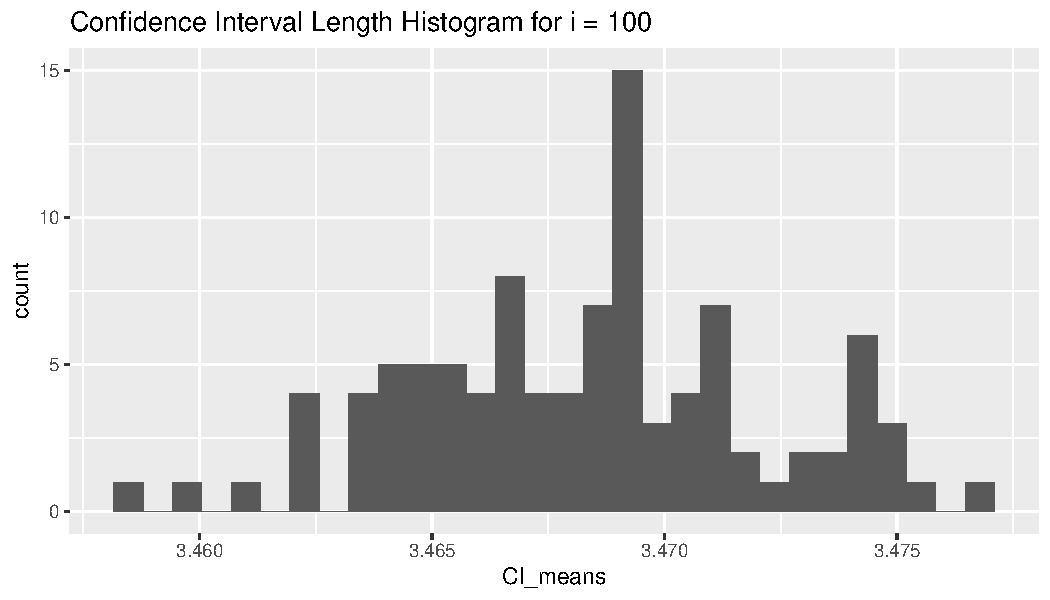
\includegraphics{report_files/figure-latex/task_2-4.pdf}
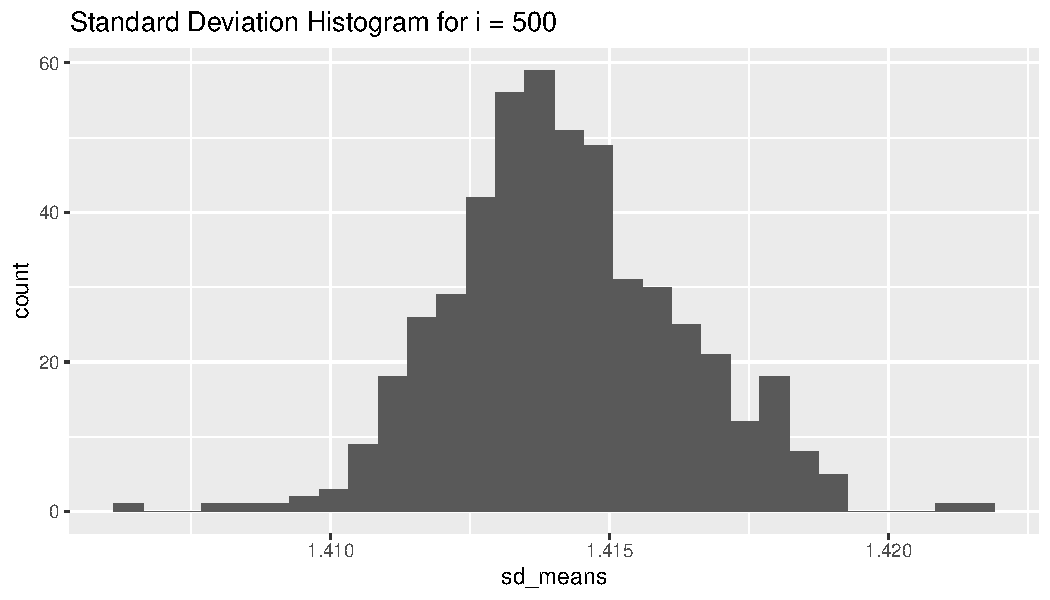
\includegraphics{report_files/figure-latex/task_2-5.pdf}
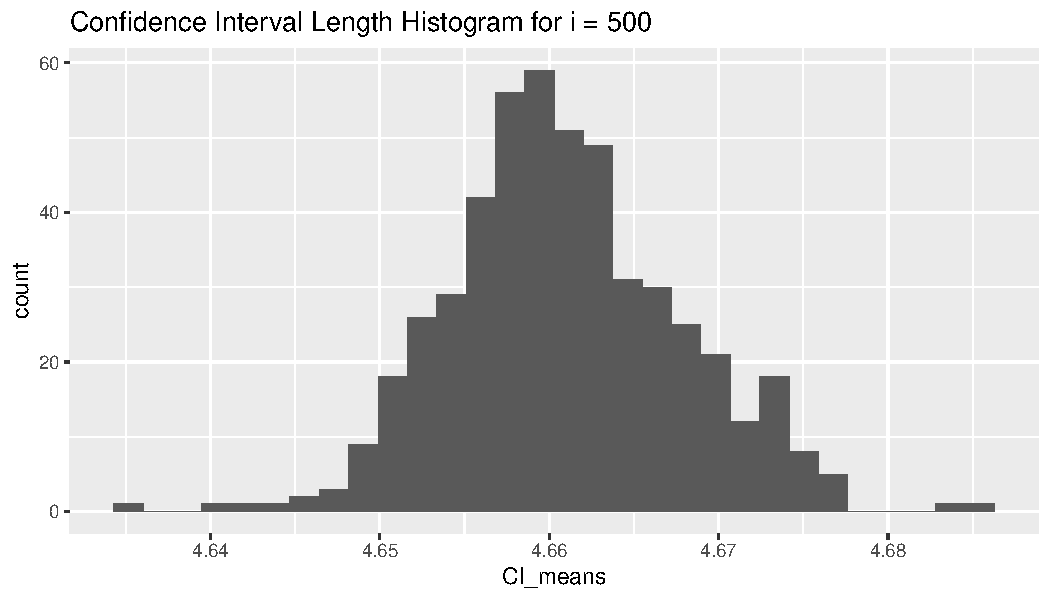
\includegraphics{report_files/figure-latex/task_2-6.pdf}
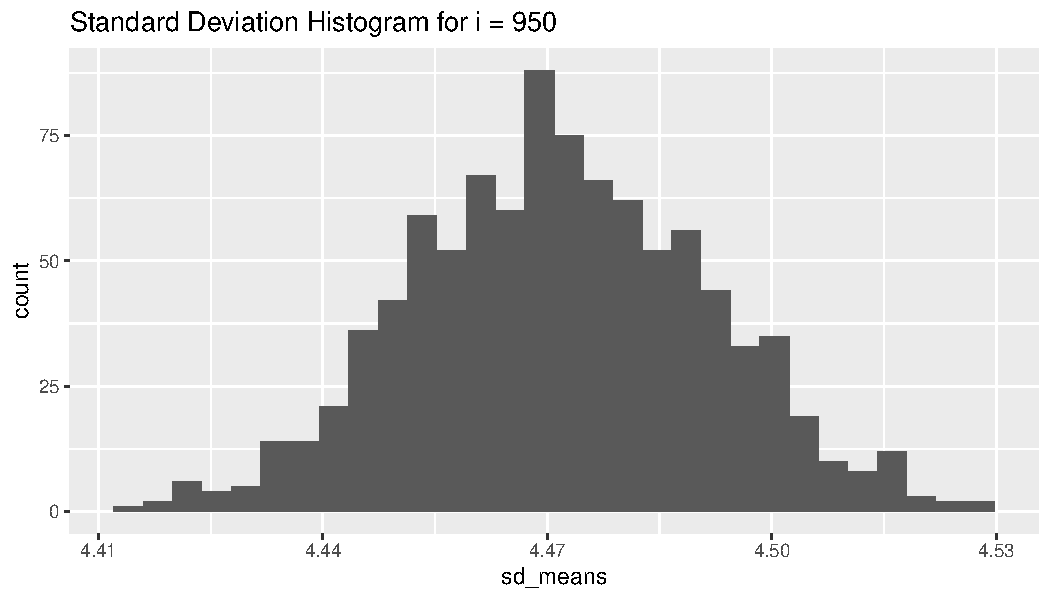
\includegraphics{report_files/figure-latex/task_2-7.pdf}
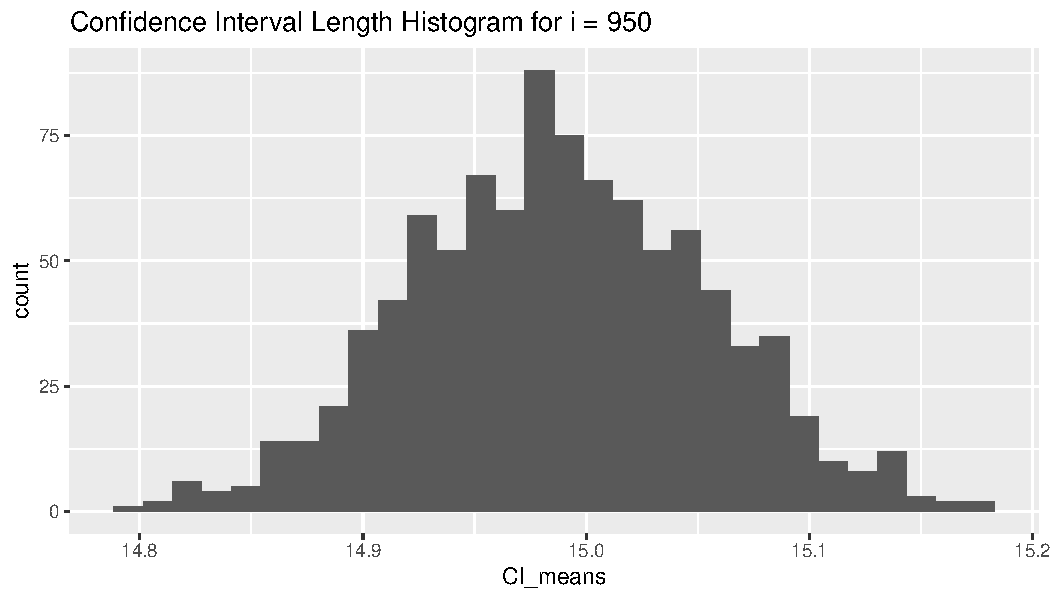
\includegraphics{report_files/figure-latex/task_2-8.pdf}

\begin{Shaded}
\begin{Highlighting}[]
\NormalTok{res <-}\StringTok{  }\KeywordTok{t}\NormalTok{(tab)}
\KeywordTok{rownames}\NormalTok{(res) <-}\StringTok{ }\KeywordTok{c}\NormalTok{(}\StringTok{"i"}\NormalTok{, }\StringTok{"sd"}\NormalTok{, }\StringTok{"CI"}\NormalTok{, }\StringTok{"FWER"}\NormalTok{,  }\StringTok{"FDR"}\NormalTok{, }\StringTok{"power"}\NormalTok{, }\StringTok{"FWER_Bonf"}\NormalTok{, }
                   \StringTok{"FDR_Bonf"}\NormalTok{, }\StringTok{"power_Bonf"}\NormalTok{,  }\StringTok{"FWER_BH"}\NormalTok{, }\StringTok{"FDR_BH"}\NormalTok{, }\StringTok{"power_BH"}\NormalTok{)}
\KeywordTok{kable}\NormalTok{(res[}\KeywordTok{c}\NormalTok{(}\StringTok{"sd"}\NormalTok{, }\StringTok{"CI"}\NormalTok{, }\StringTok{"FWER"}\NormalTok{,  }\StringTok{"FDR"}\NormalTok{, }\StringTok{"power"}\NormalTok{, }\StringTok{"FWER_Bonf"}\NormalTok{, }\StringTok{"FDR_Bonf"}\NormalTok{, }
            \StringTok{"power_Bonf"}\NormalTok{,  }\StringTok{"FWER_BH"}\NormalTok{, }\StringTok{"FDR_BH"}\NormalTok{, }\StringTok{"power_BH"}\NormalTok{),], }
      \DataTypeTok{row.names =}\NormalTok{ T, }\DataTypeTok{col.names =} \KeywordTok{c}\NormalTok{(}\StringTok{"10"}\NormalTok{, }\StringTok{"100"}\NormalTok{, }\StringTok{"500"}\NormalTok{, }\StringTok{"950"}\NormalTok{), }\DataTypeTok{digits=}\DecValTok{2}\NormalTok{)}
\end{Highlighting}
\end{Shaded}

\begin{longtable}[]{@{}lrrrr@{}}
\toprule
& 10 & 100 & 500 & 950\tabularnewline
\midrule
\endhead
sd & 1.00 & 1.05 & 1.41 & 4.47\tabularnewline
CI & 3.31 & 3.47 & 4.66 & 14.99\tabularnewline
FWER & 0.40 & 1.00 & 1.00 & 1.00\tabularnewline
FDR & 0.08 & 0.67 & 0.93 & 0.99\tabularnewline
power & 0.93 & 0.90 & 0.70 & 0.18\tabularnewline
FWER\_Bonf & 0.06 & 0.05 & 0.09 & 0.05\tabularnewline
FDR\_Bonf & 0.01 & 0.02 & 0.07 & 0.05\tabularnewline
power\_Bonf & 0.67 & 0.34 & 0.06 & 0.00\tabularnewline
FWER\_BH & 0.24 & 0.24 & 0.13 & 0.07\tabularnewline
FDR\_BH & 0.05 & 0.08 & 0.09 & 0.06\tabularnewline
power\_BH & 0.85 & 0.47 & 0.07 & 0.00\tabularnewline
\bottomrule
\end{longtable}

As we can see in the above table, adding many irrelevant variables
seriously affect the quality of the model. The standard deviation and
the confidence intervals are growing. For 945 irrelevant variables the
confidence intervals are extremally wide. Thus, in the standard approach
we are making very many discoveries. We reject almost all hypotheses. On
the other hand, using any correction causes lower power.

To summarise: including many irrelevant variables in the model leads to
low-quality model. Presented corrections can provide only limited
assistance.

\end{document}
